\documentclass[a4paper, 12p]{article}
\usepackage[spanish]{babel} 
\usepackage{amsmath} 
\usepackage[colorlinks=true]{hyperref}
\usepackage{enumitem} 
\usepackage{graphicx}   
\usepackage[a4paper,top=3cm,bottom=3cm,left=3cm,right=3cm,marginparwidth=1.75cm]{geometry} 
\usepackage[]{subfigure}
\graphicspath{{./graficos/Lab-Termo/Git/Documentos}} 
\usepackage{float}
%\usepackage[]{txfonts}
\usepackage{multicol}



\newenvironment{Figura}
{\par\medskip\noindent\minipage{\linewidth}}
{\endminipage\par\medskip}

%==================================================================================
\begin{document}
\begin{titlepage}
      \begin{center}     
            
            
\includegraphics[width=0.2\textwidth]{img/escudo_udec.png}                       %Para poner logo udec   %{nombre carpeta\nombreimagen}
            
            
            
            \vspace{1cm}
            \textsc{{\LARGE Universidad de Concepción}}
            
            \vspace{1cm}
            {\scshape\Large Facultad de ciencias fisícas y matemáticas \par}
            \vspace{2cm}
            {\scshape\Huge Laboratorio 4 \par}
            \vspace{2cm}
            {\itshape\Large Proyecto laboratorio termodinámica \par}
            \vfill
            {\Large Autores: \par}
            {\Large Martina Contreras, Noemí De La Peña, Benjamín Opazo. \par}
            \vfill
            \vfill
            {\Large Profesor: \par}
            {\Large Claudio Alonso Faúndez Araya \par}
            \vfill
            \vfill
            {\Large Carrera: \par}
            {\Large Ciencias fisícas \par}
            \vfill
            \vfill
            {\Large Ayudante: \par}
            {\Large Renata Hernández Lopez \par}
            \vfill
            {\Large Noviembre 2022 \par}
      \end{center}
\end{titlepage}            


\tableofcontents
\newpage

%========Introducción
\section{Introducción}
En este informe presentaremos la experiencia del laboratorio, cuya finalidad fue la calcular la densidad de aceite de cocina por medio del ley de la hidrostática. primero presentaremos los objetivos del laboratorio, para luego definir conceptos importantes, tales como, que es la ley de la hidrostática y la densidad. Luego, responderemos las preguntas propuestas en el análisis. Para finalizar, anunciaremos si los objetivos se lograron cumplir junto con la veracidad de nuestra hipótesis.

\section{Objetivos}
\begin{itemize}
      \item Determinar la densidad de aceite de cocina por medio de la ley de la Hidrostática.
      
      \item Comparar el valor determinado con el de literatura.
\end{itemize}



%=========Marco Teórico
\section{Marco Teórico} 
\section*{Presión y densidad}
La presión es una magnitud física intensiva que corresponde a la distribución de fuerza que se ejerce sobre una superficie. En este caso se considera que esta fuerza es debida a un fluido. 
Esta fuerza tiene orientación normal respecto de dicha superficie. Esta superficie puede ser una pared sólida, como las paredes de un contenedor, ó una superficie imaginaria que delimita una 
región en el interior de un volumen de fluido ó un cambio de fase (distintos fluidos inmiscibles). Este último caso corresponde a la presión interna del fluido. En términos generales, 
corresponde a una intensidad de carga sobre un punto de una superficie, depende del punto. En el caso de que la distribución de la fuerza sea uniforme, como una superficie plana con un fluido homogéneo, 
entonces la presión es constante en toda la superficie. Esta magnitud se mide en Pascales $[Pa]$.

La densidad $\rho$ de una sustancia, cualquiera sea su estado, corresponde una relación entre el volumen de ella y la cantidad de materia que contiene. Sus unidades de medida son $kg/m³$, en el SI. En el caso particular de un fluido, 
presenta variaciones pequeñas ante cambios de temperatura y presión en el tiempo, por lo que, para efectos prácticos, su densidad no cambia (fluido incompresible).

\subsection*{Ley de la hidroestática}
Si se agrega que la densidad del fluido en estudio es homogénea (es la misma en cualquier región al interior de él), que se encuentra en reposo y que sobre su superficie superior se ejerce una presión $P_0$, entonces, a una profundidad $h$, 
medida desde dicha superficie en dirección de $\vec{g}$, la presión allí, $P$, es dada por la ley de la hidroestática.
\begin{align}
      P=P_0 +  \rho gh.
      \label{eq: presion-h}
\end{align}

Dados dos fluidos inmiscibles estáticos, pueden ordenarse de forma tal que puede determinarse la densidad de uno dada la del otro, por ejemplo, teniendo agua, de densidad $\rho_ag = 1000[kg/m³]$, y aceite con densidad $\rho_ac$ desconocida.


\newpage
%=========Materiales
\section{Materiales}


\begin{itemize}
      \item 1 tubo en U.
      \item 1 soporte universal.
      \item 2 pinzas de sujeción.
      \item Regla escuadra.
      \item Aceite de cocina.
      \item agua,
\end{itemize}    




\begin{figure}[H]
      \begin{subfigure}
            \raggedright
            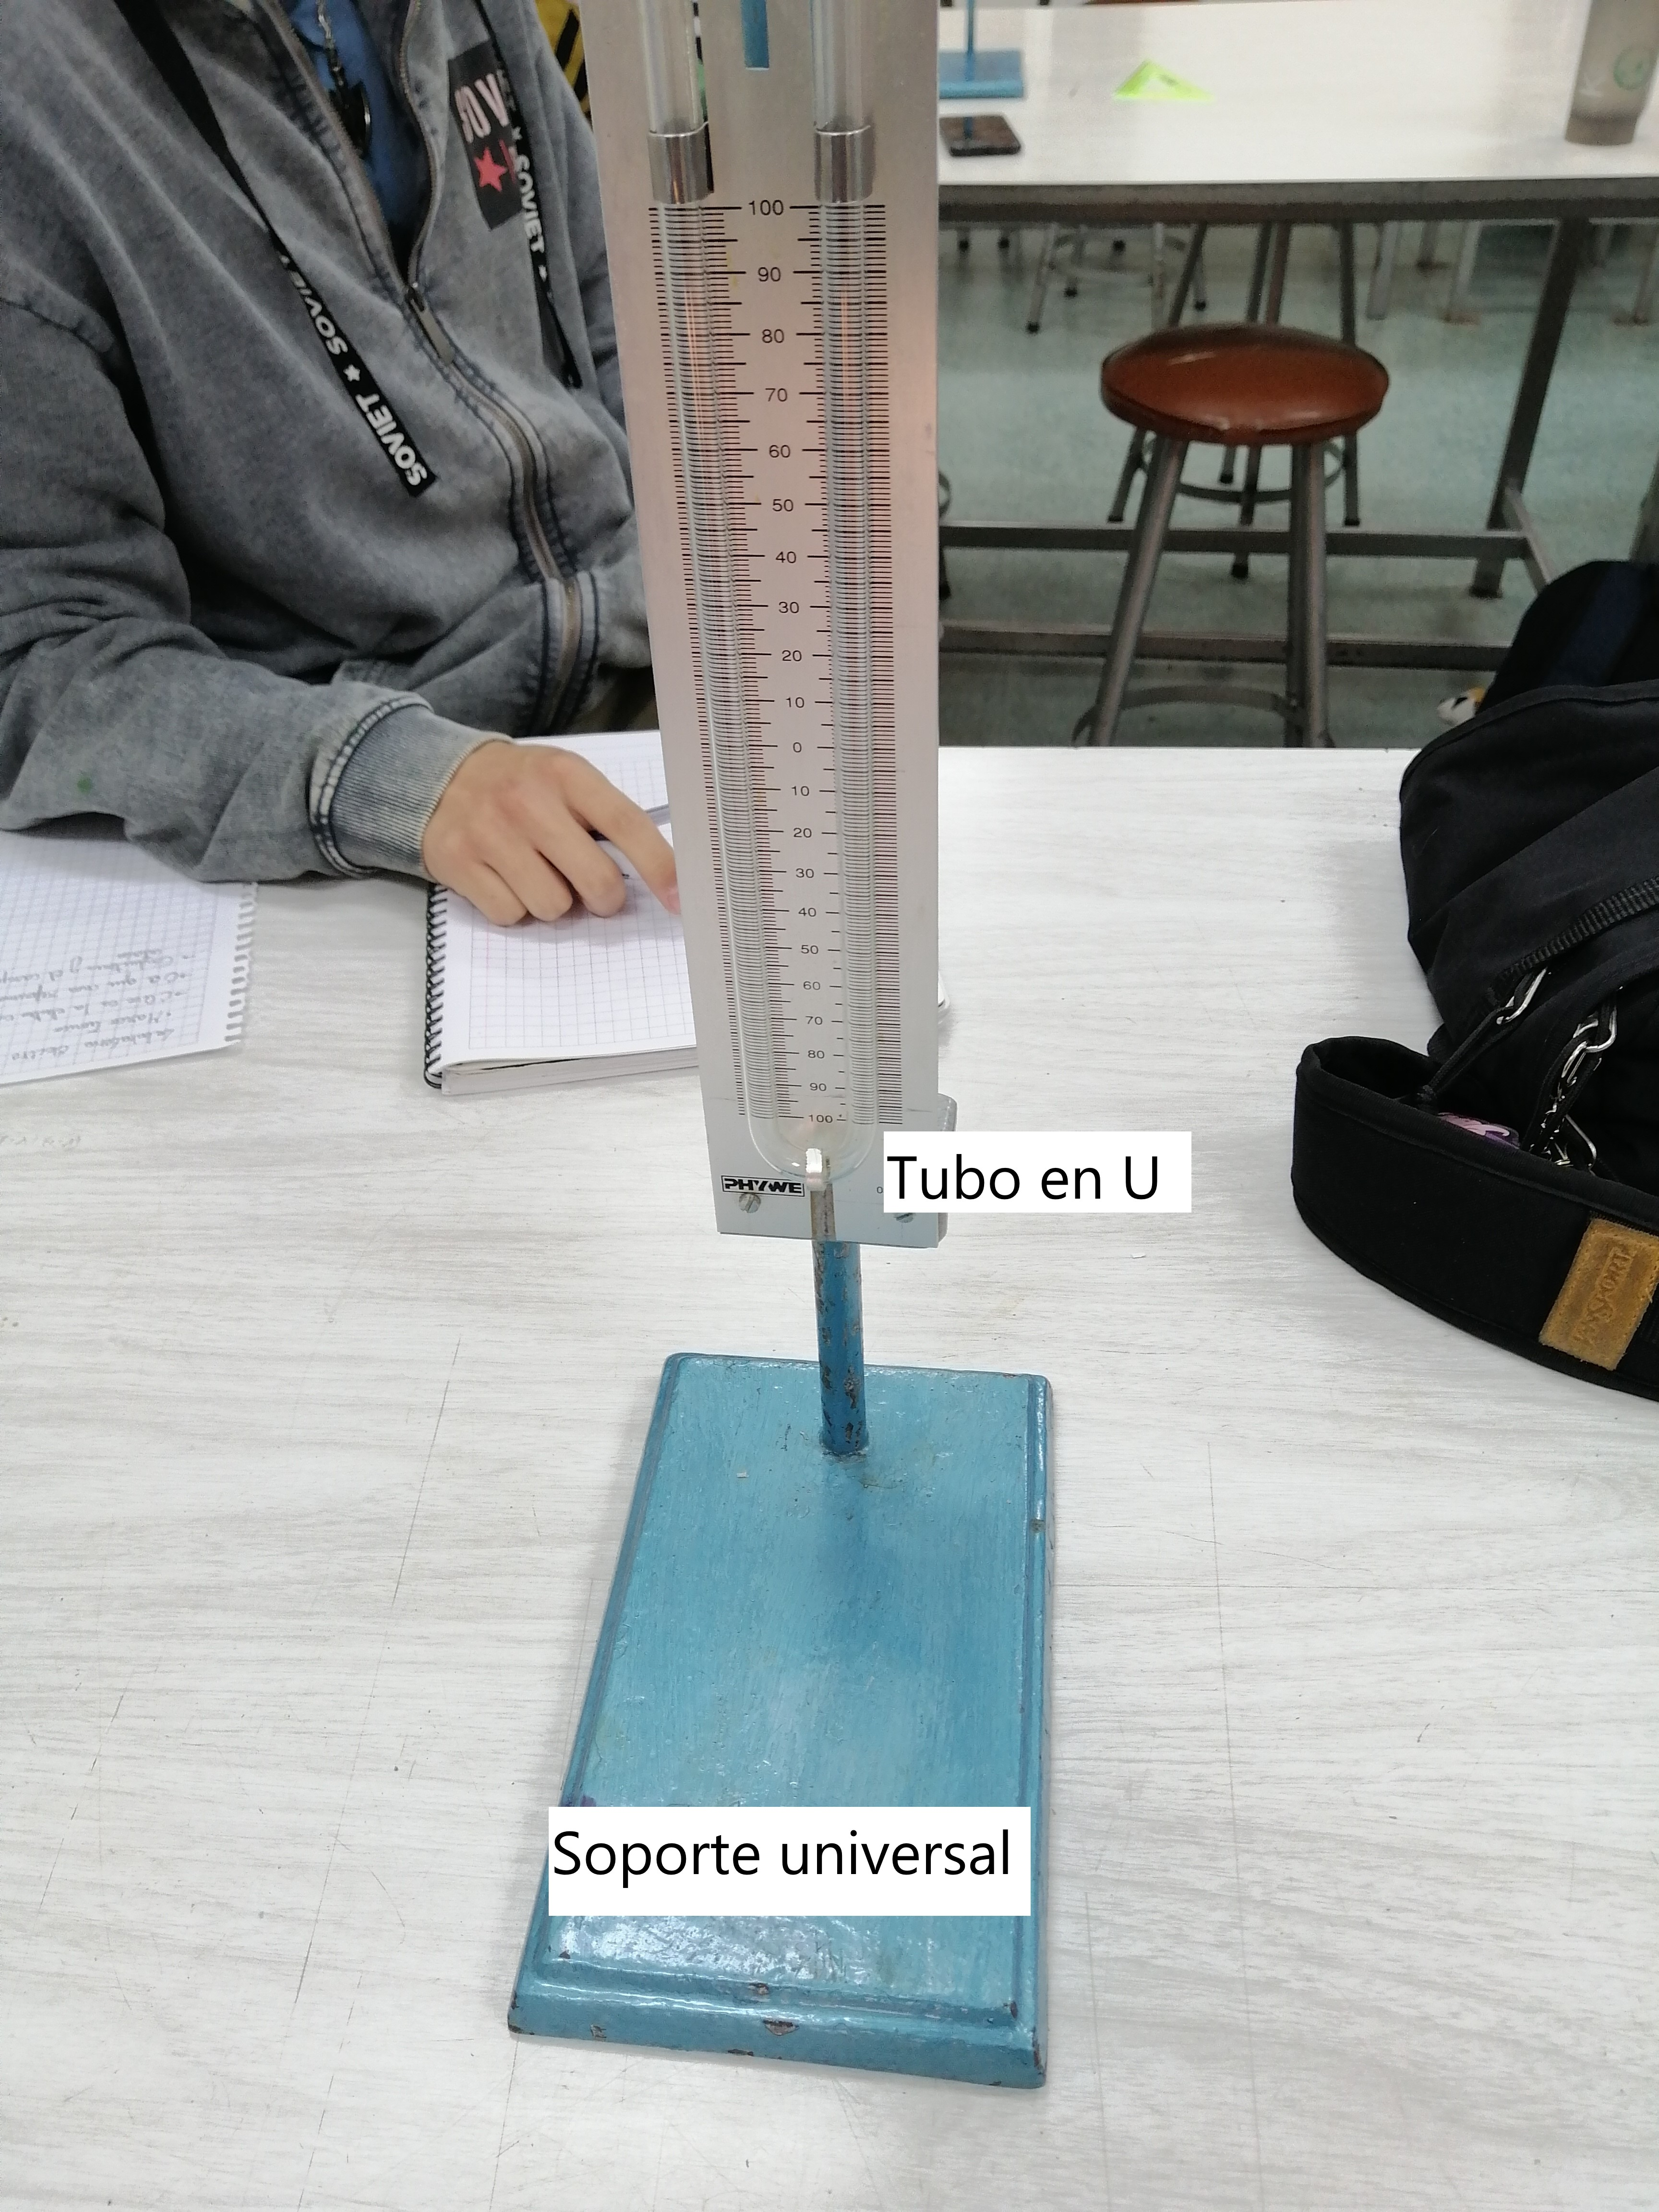
\includegraphics[width=6cm, height=6.5cm]{img/image2.jpg}
      \end{subfigure}
      \begin{subfigure}
            \centering
            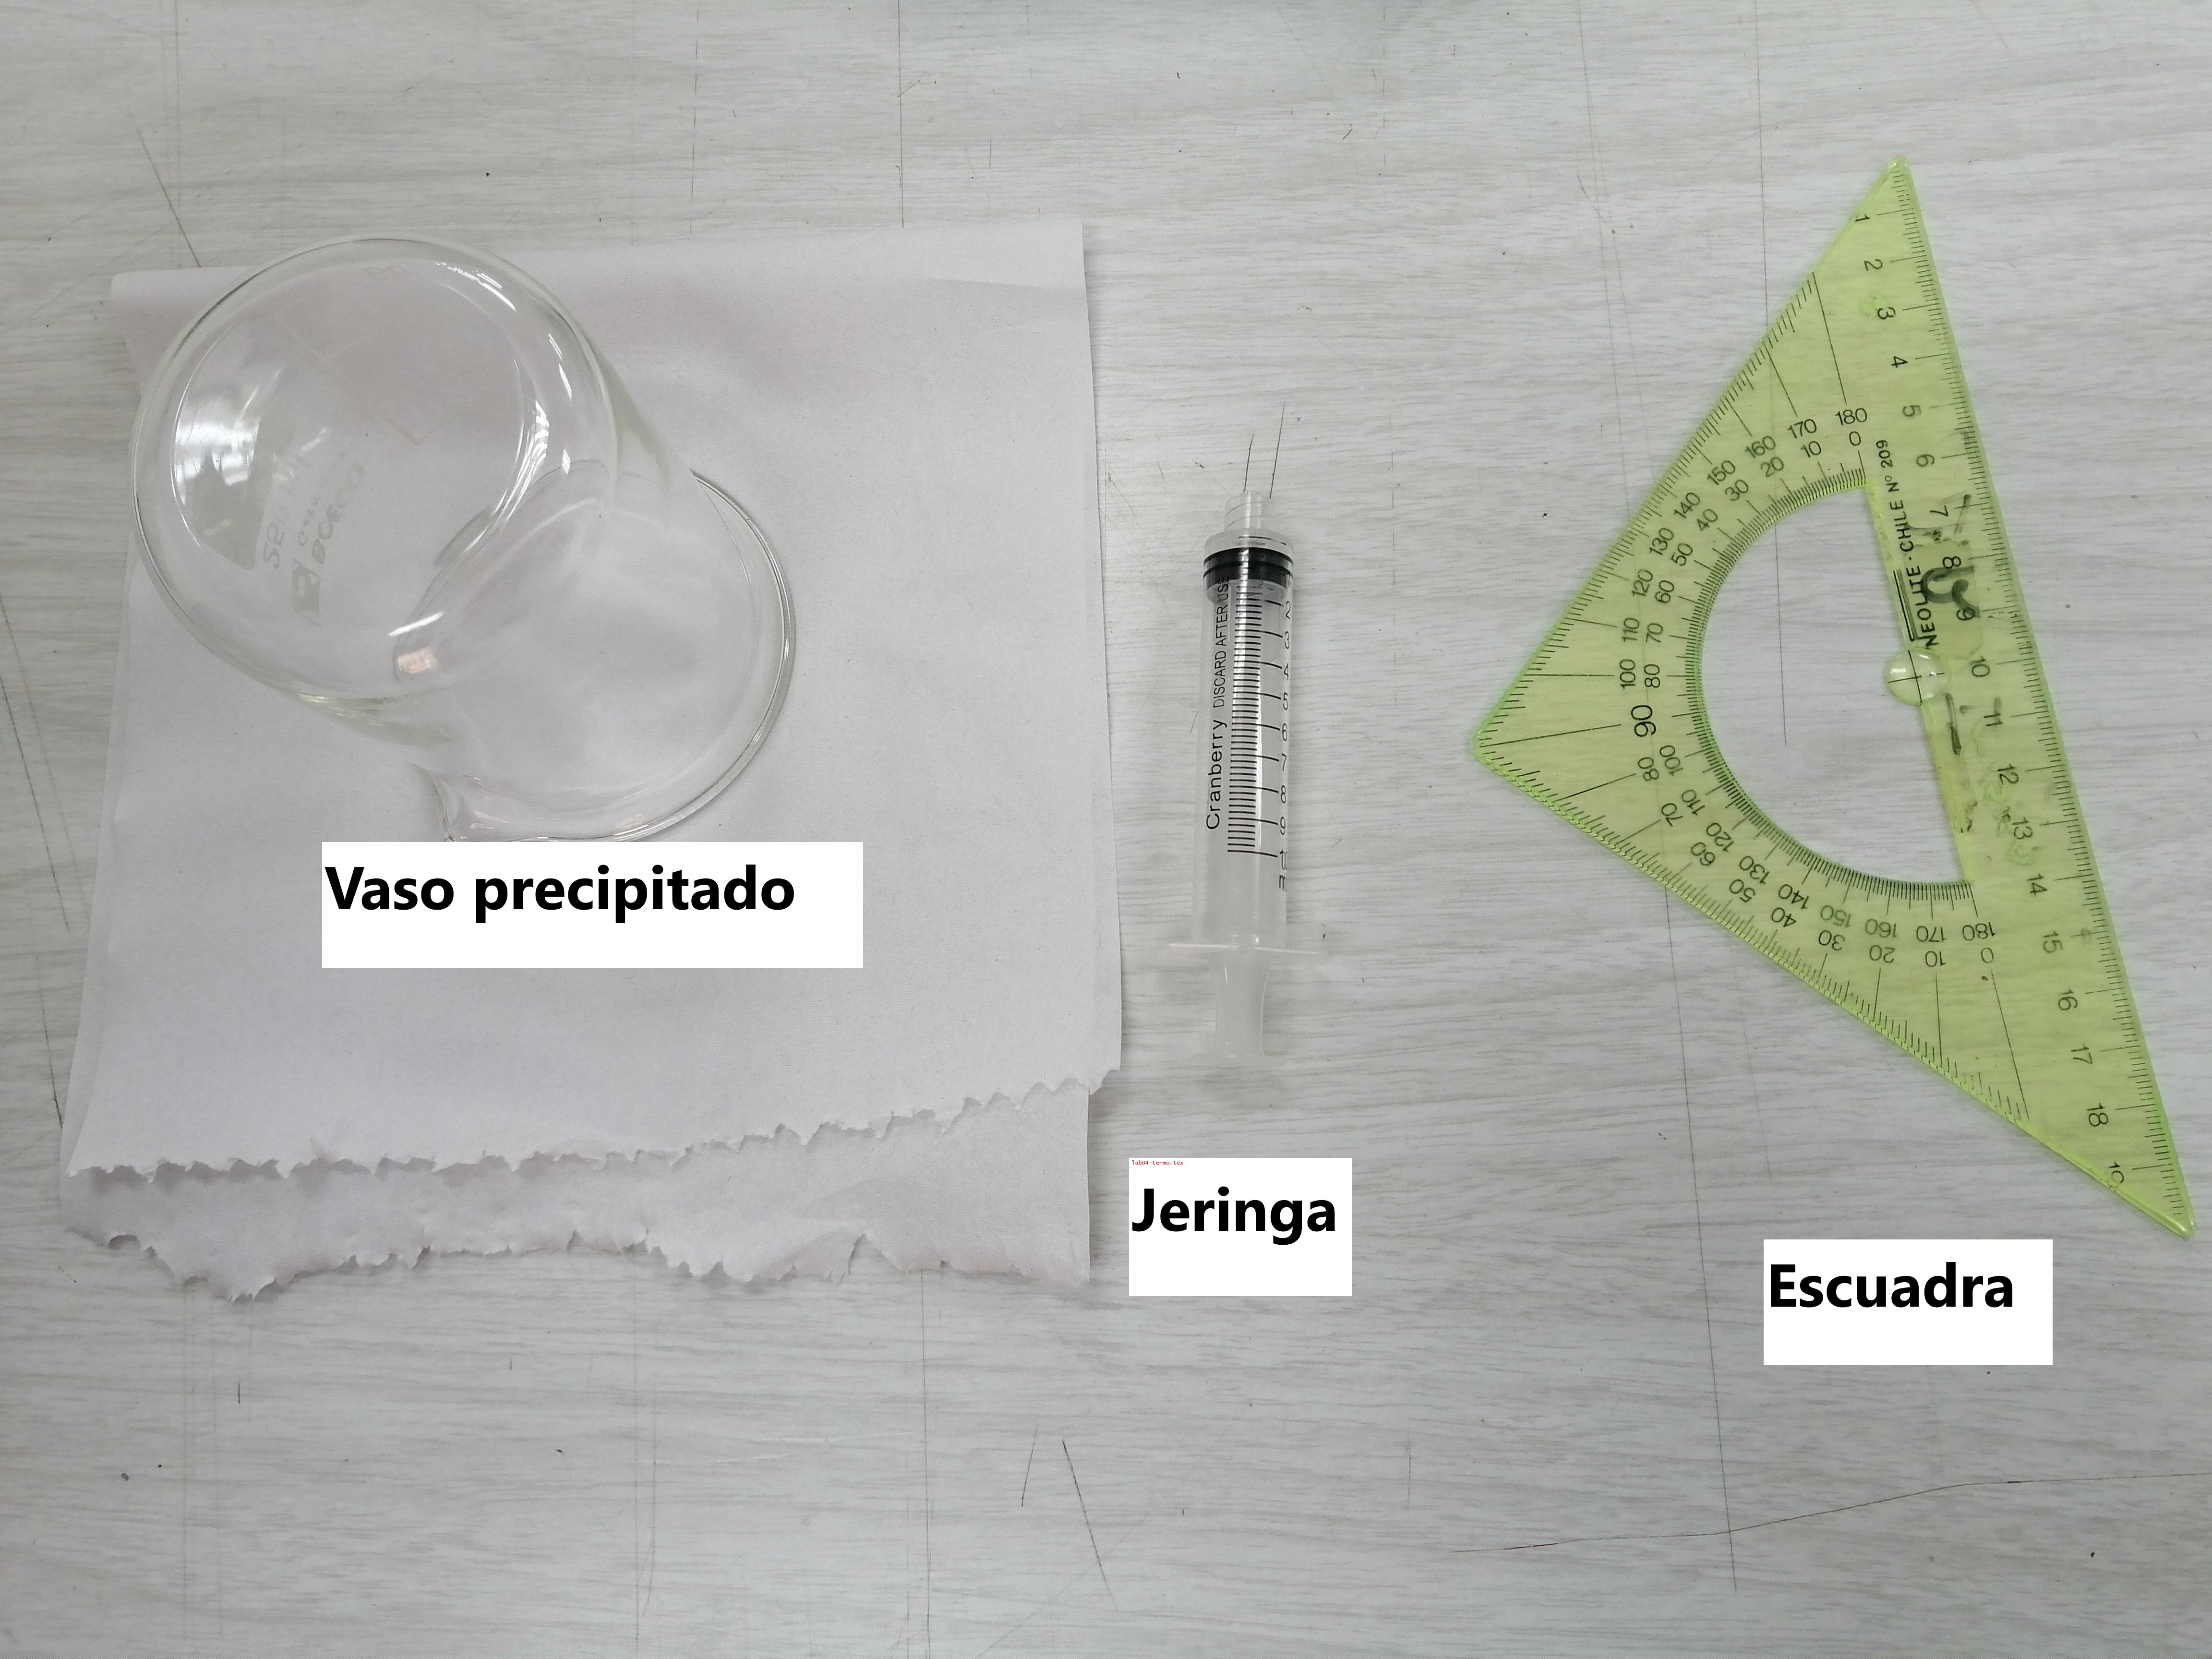
\includegraphics[width=4.5cm, height=4.5cm]{img/image1.jpg}   
      \end{subfigure}  
      \begin{subfigure}
            \raggedleft
            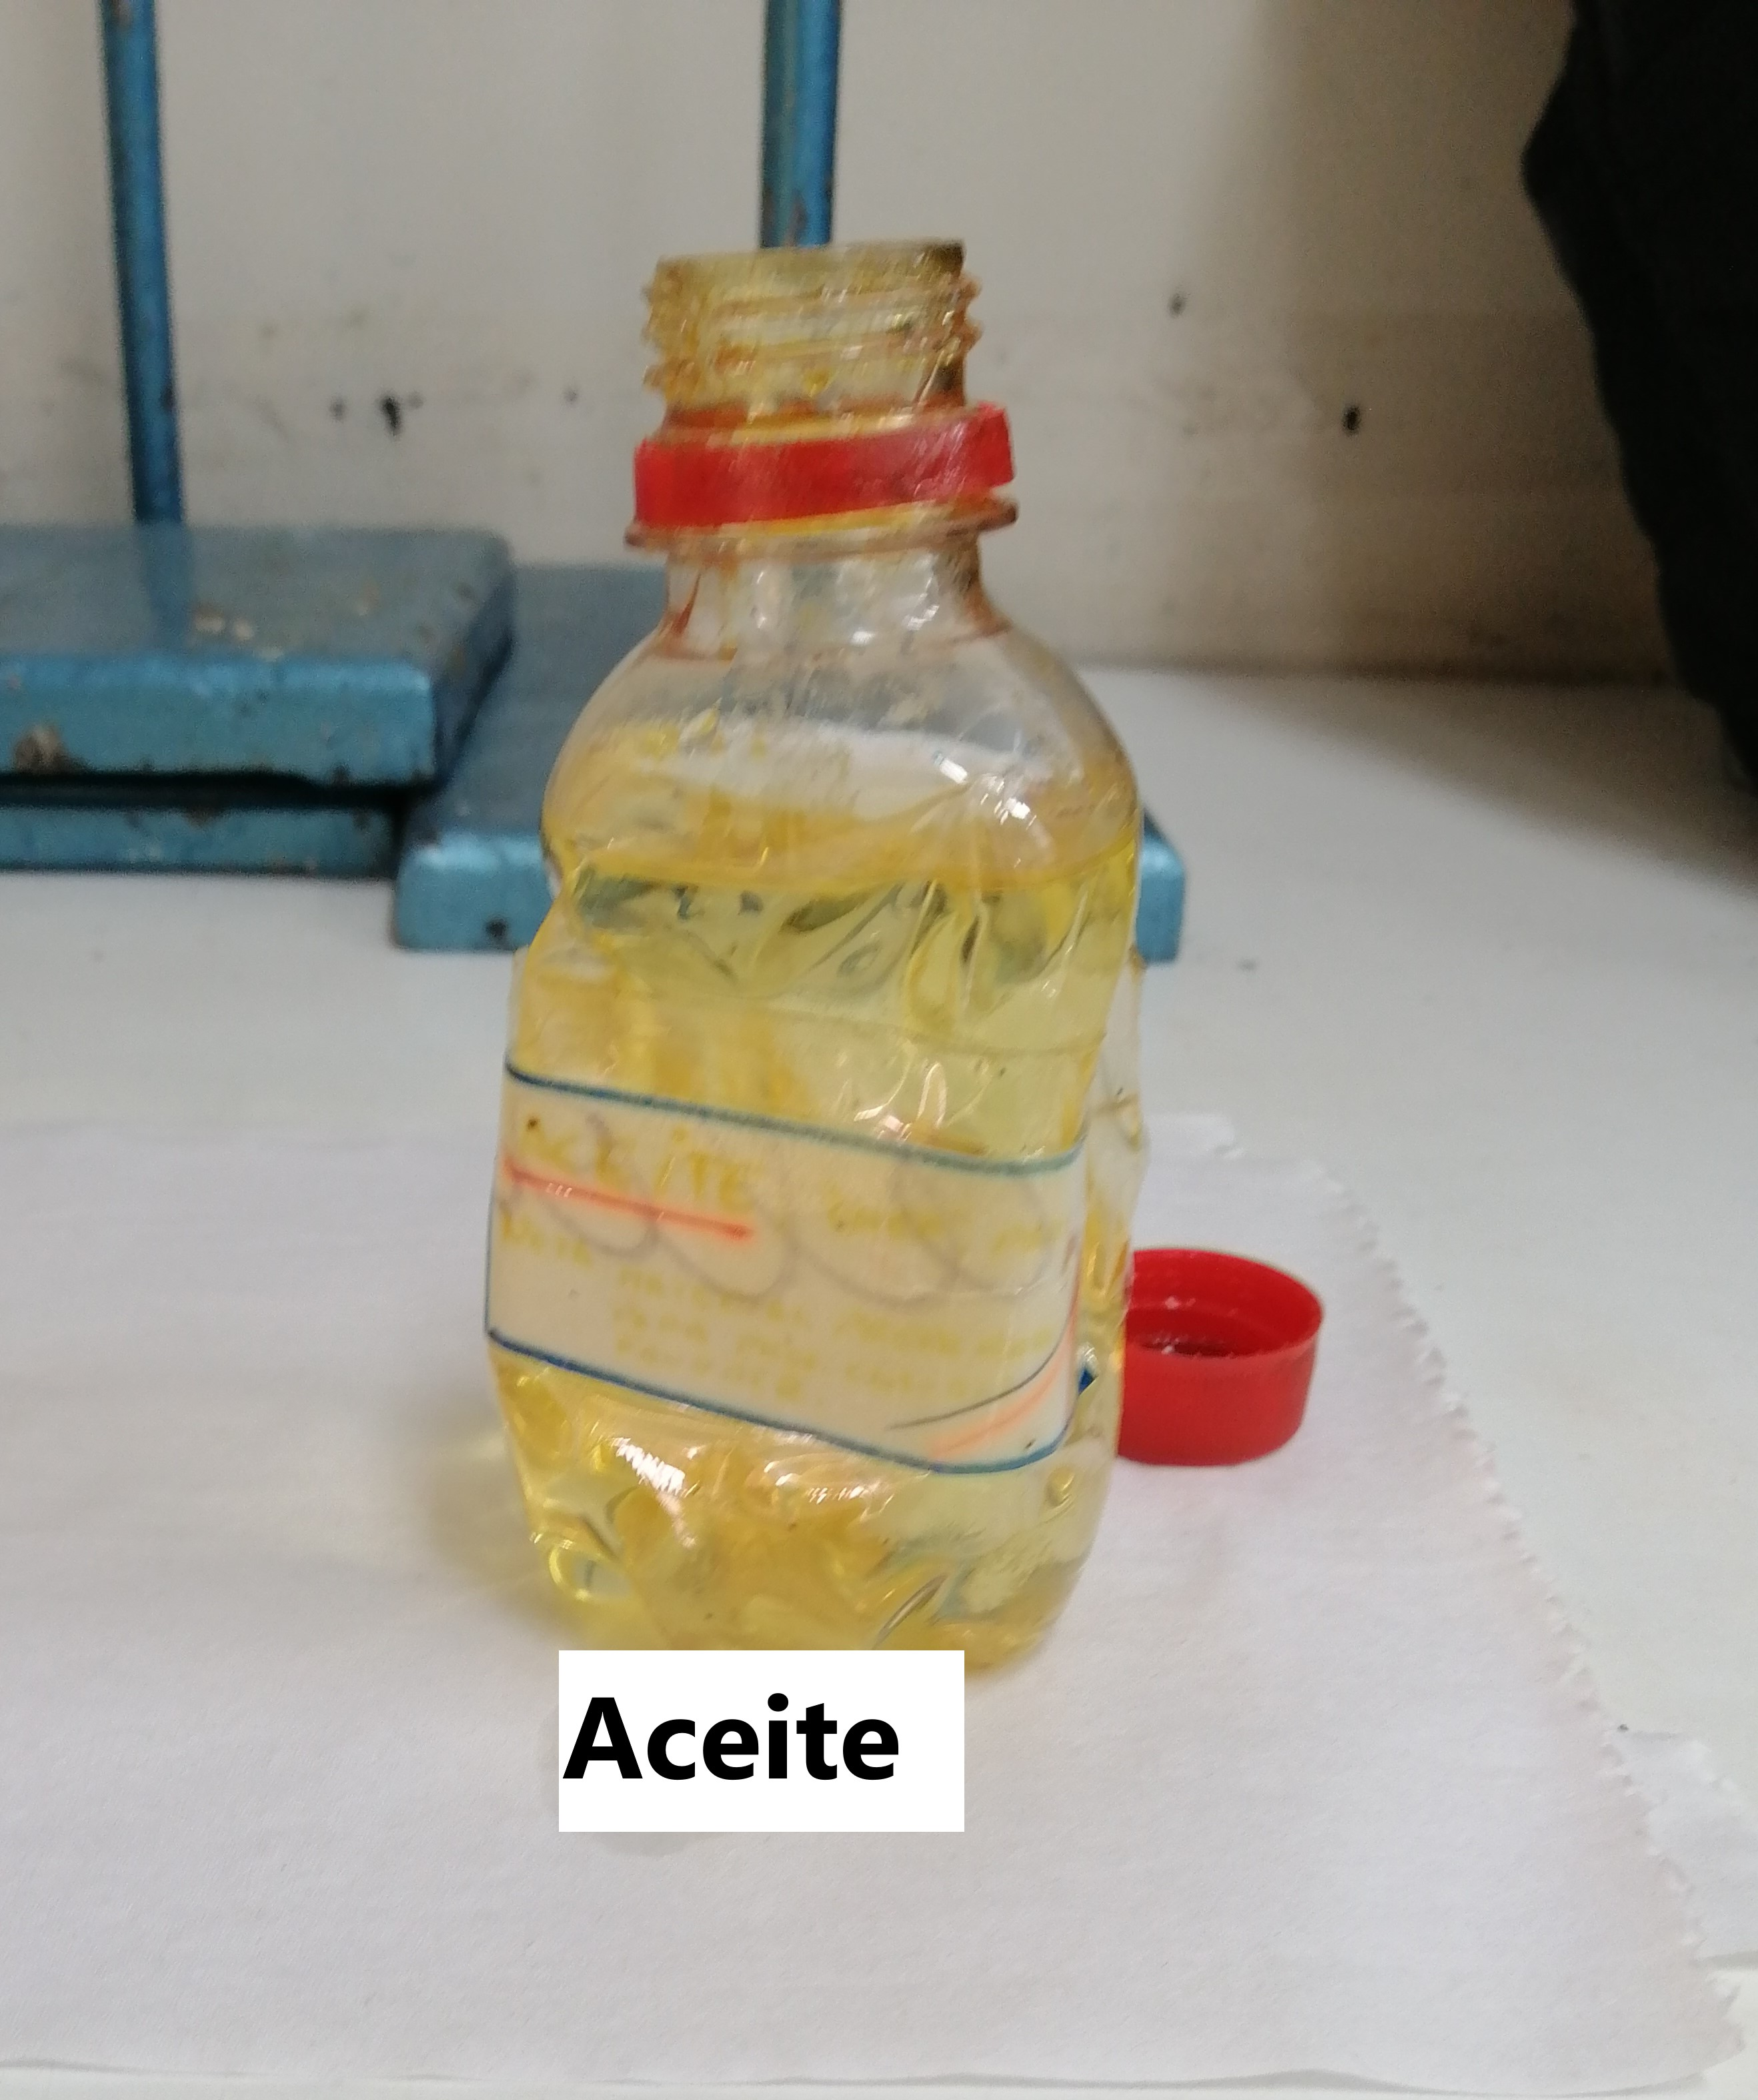
\includegraphics[width=4cm, height=4cm]{img/image3.jpg}
      \end{subfigure}
\end{figure}



\section{Procedimiento}

\begin{itemize}
      \item Primero debemos llenar el tubo en u con $8[cc]$ de agua.
      
      \item Luego agregamos $4[cc]$ de aceite de cocina por algunas de las ramas del tubo en u.
      
      \item Medir las alturas mostradas en la Fig.1 para calcular la altura de cada una de las columnas.
      
\end{itemize}

\section{Análisis}
\begin{itemize}
      \item Usando la ley de la Hidroestática, calcular la presión hidroestática en el nivel de referencia $h_{0}$ y obtener la expresión que relaciona esta presión con la densidad del aceite.\\ 
      R: Primero nuestros datos son:\\
      P es la presión hidroestática.\\
      $P_{0}$ es la presion atmosférica $1.013 \times 10^5 N/m^2$.\\
      $\rho$ es la densidad del líquido, en nuestro caso la del agua $1000 kg/m^3$.\\
      $h$ es la altura, que es medida desde donde empieza el líquido hasta un punto B, la cual es $0.13m$\\
      $g$ es la aceleración de gravedad $9.8 m/s^2$.\\
      
      Utilizando la ley de la Hidroestática \ref{eq: presion-h} y reemplazando nuestros datos, tenemos que:

       \begin{equation*}
       P = 1.013 \times 10^5\dfrac{N}{m^2} + 1000\dfrac{kg}{m^3} \times 0.13m \times 9.8\dfrac{m}{s^2}
       \end{equation*}
       Y así obtenemos que la presión hidroestática es: 
       \begin{equation*}
       P = 102574 \dfrac{N}{m^2}  
       \end{equation*}
      
      \item Calcular la densidad del aceite.\\
      R: Si tomamos dos puntos a una misma altura sus presiones serán las mismas, por lo que tenemos una igualdad de presiones, tal que:
      \begin{equation*}
      P_{B} = P_{A}
      \end{equation*}            
      ,donde A y B son puntos del tubo en U, donde B está en el agua y A en el aceite, así tenemos que
      \begin{equation}\label{eq2}
      P_{0} +  \rho_{ag} h_{ag} g = P_{0} +  \rho_{ac} h_{ac} g  
      \end{equation}
      Donde nuestros datos son:\\
      $P_{0}$ es la presion atmosférica $1.013 \times 10^5 N/m^2$.\\
      $\rho_{ag}$ es la densidad del agua $1000 kg/m^3$.\\
      $\rho_{ac}$ es la densidad del aceite, la cual es la incógnita.\\
      $h_ag$ es la altura, que es medida desde donde empieza el agua hasta un punto B, la cual es $0.13m$\\
      $h_{ac}$ es la altura, que es medida desde donde empieza el aceite hasta un punto A, la cual es $0.14m$.\\
      $g$ es la aceleración de gravedad $9.8 m/s^2$.\\
     
      Reemplazando nuestros datos en \ref{eq2}, tenemos que
      \begin{equation}\label{eq3}
      1.013 \times 10^5\dfrac{N}{m^2} + 1000\dfrac{kg}{m^3} \times 0.13m \times 9.8\dfrac{m}{s^2} = 1.013 \times 10^5\dfrac{N}{m^2} +  \rho_{ac} \times 0.14m \times 9.8\dfrac{m}{s^2}  
      \end{equation}
      Despejando $\rho_{ac}$ de \ref{eq3}, tenemos que 
      \begin{equation*}
      \rho_{ac} = 928.57\dfrac{kg}{m^3}
      \end{equation*}
      
      \item Comparar el resultado obtenido con valores de referencia encontrados en la literatura por medio del error porcentual $\epsilon_{r}$,
      \begin{equation}\label{eq4}
      \epsilon_{r} = \left|\dfrac{\rho_{ac,r} - \rho_{ac,ex}}{\rho_{ac,r}} \right| \times 100 \% ,
      \end{equation}
      donde $\rho_{ac,r}$ es la densidad del aceite de referencia y $\rho_{ac,ex}$ es el valor calculado en este experimento.
      R: Tomaremos a $\rho_{ac,r}$  igual a $920 kg/m^3$, el cual fue obtenido de \ref{eq: presion-h}, ahora reemplazanpo nuestros valores en \ref{eq4}, tenemos que:
      \begin{equation*}
      \epsilon_{r} = \left|\dfrac{ 920 kg/m^3 - 928.57 kg/m^3}{920 kg/m^3} \right| \times 100 \%
      \end{equation*}
       Así obtenemos que $\epsilon_{r} = 0.93 \%$
     
     \end{itemize}
\section{Conclusión}

Al finalizar este informe, podemos decir que los objetivos se cumplieron. Calculamos la presión hidrostática que relaciona la densidad del aceite y con esta forma calcular el valor de la densidad del aceite.

Luego calculamos el error relativo proveniente de la densidad del aceite, calculada en el experimento, junto con la densidad del aceite proveniente en la literatura. Dándonos un valor sumamente pequeño, es decir, es bastante fiable utilizar la ley de la hidrostática para calcular densidades.
concluir que:
Es posible calcular, aproximadamente, cualquier densidad, a través de la ley de la hidrostática, reafirmando nuestra hipótesis anteriormente planteada.






% \begin{thebibliography}{6}
      %       \bibitem{libro} Sears, F. W., Salinger, G. L. \& Peris, A. J. (2021, 10 enero). Termodinámica, teoría cinética y termodinámica estadística (Spanish Edition) (1.a ed.). Reverte.
      %       \bibitem{profe} Faundez Araya, C. A. (s. f.). Capítulo 3. Primer Principio de la Termodinámica [Diapositivas]. Universidad de Concepción, 2022.
      %       \bibitem{agua}Fundación Aquae. (2021, 10 agosto). CP del agua: significado y valores - Fundación Aquae. FundaciÃ3n Aquae. 
      %       \url{https://www.fundacionaquae.org/wiki/cp-del-agua/}
      %       \bibitem{acero}DeterminaciÃ3n del calor específico de un sÃ3lido. (s. f.). Recuperado 25 de octubre de 2022,
      %       de \url{http://www.sc.ehu.es/sbweb/fisica/estadistica/otros/calorimetro/calorimetro.htm}
      % \end{thebibliography}
      
      
      
      
      
      
      
      
      
      
      
      
      
      \end{document}
      